% !TEX program = pdflatex
\documentclass[aspectratio=169, 10pt]{beamer}

%% ============================================================
%% PACKAGES
%% ============================================================
\usepackage[T1]{fontenc}
\usepackage{lmodern}
\usepackage{graphicx}
\usepackage{booktabs}
\usepackage{array}
\usepackage{tabularx}
\usepackage{colortbl}
\usepackage{tikz}
\usetikzlibrary{positioning, calc, arrows.meta, shapes.geometric, fit, shadows}
\usepackage[most]{tcolorbox}
\usepackage{fontawesome5}
\usepackage{hyperref}
\usepackage{pgfplots}
\pgfplotsset{compat=1.18}
\usepackage{multicol}
\usepackage{xcolor}
\usepackage{textcomp}
\usepackage{pifont}

\graphicspath{{figures/}}

%% ============================================================
%% COLOR DEFINITIONS
%% ============================================================
\definecolor{UVMGreen}{HTML}{154734}
\definecolor{UVMGold}{HTML}{D4A84B}
\definecolor{SlateTeal}{HTML}{1B4D5C}
\definecolor{DeepCharcoal}{HTML}{2C3E50}
\definecolor{SoftCoral}{HTML}{C0534D}
\definecolor{CoolGray}{HTML}{8899A6}
\definecolor{PaleSage}{HTML}{EDF2F0}
\definecolor{LightGold}{HTML}{FDF6E3}
\definecolor{DarkSlate}{HTML}{0F2B36}
\definecolor{AccentBlue}{HTML}{3498DB}

%% ============================================================
%% BEAMER THEME SETUP
%% ============================================================
\setbeamercolor{structure}{fg=SlateTeal}
\setbeamercolor{normal text}{fg=DeepCharcoal}
\setbeamercolor{frametitle}{fg=SlateTeal}
\setbeamercolor{title}{fg=SlateTeal}
\setbeamercolor{subtitle}{fg=UVMGold}
\setbeamercolor{author}{fg=DeepCharcoal}
\setbeamercolor{date}{fg=CoolGray}
\setbeamercolor{institute}{fg=CoolGray}
\setbeamercolor{footline}{fg=CoolGray}
\setbeamercolor{block title}{fg=white, bg=SlateTeal}
\setbeamercolor{block body}{bg=PaleSage}
\setbeamercolor{alerted text}{fg=SoftCoral}
\setbeamercolor{item}{fg=SlateTeal}
\setbeamercolor{subitem}{fg=CoolGray}

\setbeamerfont{title}{size=\Large, series=\bfseries}
\setbeamerfont{subtitle}{size=\normalsize}
\setbeamerfont{frametitle}{size=\large, series=\bfseries}
\setbeamerfont{footline}{size=\tiny}

\setbeamertemplate{navigation symbols}{}

% Custom frame title
\setbeamertemplate{frametitle}{%
  \vskip14pt%
  \nointerlineskip%
  {\usebeamerfont{frametitle}\usebeamercolor[fg]{frametitle}\insertframetitle\par}%
  \vskip2pt%
  {\color{UVMGold}\rule{\textwidth}{1.2pt}}%
  \vskip3pt%
}

% Custom footline
\setbeamertemplate{footline}{%
  \begin{beamercolorbox}[wd=\paperwidth, ht=16pt, right, rightskip=1.5cm]{footline}%
    \usebeamerfont{footline}\insertframenumber\,/\,\inserttotalframenumber\vskip3pt%
  \end{beamercolorbox}%
}

% Itemize styles
\setbeamertemplate{itemize item}{\color{SlateTeal}\raisebox{0.15ex}{\small$\blacktriangleright$}}
\setbeamertemplate{itemize subitem}{\color{CoolGray}\raisebox{0.1ex}{\footnotesize$\bullet$}}

% Compact tcolorbox defaults
\tcbset{
  keybox/.style={
    colback=PaleSage, colframe=SlateTeal, boxrule=0.8pt, arc=3pt,
    left=6pt, right=6pt, top=4pt, bottom=4pt,
    fonttitle=\bfseries\small\color{white}, coltitle=white, colbacktitle=SlateTeal,
  },
  accentbox/.style={
    colback=LightGold, colframe=UVMGold, boxrule=0.8pt, arc=3pt,
    left=6pt, right=6pt, top=4pt, bottom=4pt,
  },
  quotebox/.style={
    colback=PaleSage, colframe=SlateTeal!50, boxrule=0.5pt, arc=2pt,
    left=8pt, right=8pt, top=4pt, bottom=4pt,
    borderline west={3pt}{0pt}{UVMGold},
  },
}

%% ============================================================
%% METADATA
%% ============================================================
\title{Agentic AI Bootcamp}
\subtitle{Research Workflows \& Code Auditing}
\author{Erkmen G. Aslim \and Emily Beam}
\institute{Department of Economics, University of Vermont}
\date{April 27, 2026}

\begin{document}

%% ====== SLIDE 1: TITLE ======
{
\setbeamertemplate{footline}{}
\begin{frame}[plain]
\begin{tikzpicture}[remember picture, overlay]
  % SlateTeal background
  \fill[SlateTeal] (current page.north west) rectangle (current page.south east);
  % Gold accent line across the middle
  \fill[UVMGold] ([yshift=0.3cm]current page.center -| current page.west) rectangle ([yshift=0.25cm]current page.center -| current page.east);
  % Title block (above the line)
  \node[anchor=center, text=white, font=\fontsize{28}{34}\bfseries\selectfont]
    at ([yshift=2.2cm]current page.center) {Agentic AI Bootcamp};
  \node[anchor=center, text=UVMGold, font=\fontsize{15}{20}\selectfont]
    at ([yshift=1.2cm]current page.center) {Research Workflows \& Code Auditing};
  % Instructor names (below the line, prominent)
  \node[anchor=center, text=white, font=\large\bfseries]
    at ([yshift=-0.6cm]current page.center) {Erkmen G. Aslim \quad\&\quad Emily Beam};
  \node[anchor=center, text=PaleSage, font=\normalsize]
    at ([yshift=-1.3cm]current page.center) {Department of Economics, University of Vermont};
  % Date and location
  \node[anchor=center, text=CoolGray!70!white, font=\small]
    at ([yshift=-2.2cm]current page.center) {Session 2 \quad$\cdot$\quad April 27, 2026 \quad$\cdot$\quad Old Mill A500};
  \node[anchor=center, text=UVMGold, font=\small\ttfamily]
    at ([yshift=-2.8cm]current page.center) {eabeam.github.io/uvmecon-ai};
  % Subtle robot watermark
  \node[text=white, opacity=0.04, font=\fontsize{100}{100}\selectfont, anchor=center, rotate=-15]
    at ([xshift=5cm, yshift=1.5cm]current page.center) {\faRobot};
\end{tikzpicture}
\end{frame}
}

%% ====== SLIDE 2: AGENDA ======
\begin{frame}{What We'll Cover Today}
\begin{columns}[T]
\begin{column}{0.47\textwidth}
\begin{tcolorbox}[keybox, title={\faFlask\quad Emily: Research Workflows}]
\small
\begin{itemize}\setlength{\itemsep}{2pt}
  \item Data exploration pipeline
  \item Live demo: Lead in Vermont
  \item Code auditing a replication package
  \item Paper auditing with \texttt{/econ-audit}
  \item AI vs.\ real referee reports
\end{itemize}
\end{tcolorbox}
\end{column}
\begin{column}{0.47\textwidth}
\begin{tcolorbox}[keybox, title={\faGlobe\quad Erkmen: Data \& Grading}]
\small
\begin{itemize}\setlength{\itemsep}{2pt}
  \item Web scraping with AI
  \item Automated grading feedback
  \item Hands-on practice time
\end{itemize}
\end{tcolorbox}
\end{column}
\end{columns}
\end{frame}

%% ====== SLIDE 3: SESSION 1 RECAP + TODAY'S FRAME ======
\begin{frame}{From Chat to Workflows}
\begin{columns}[T]
\begin{column}{0.47\textwidth}
\begin{tcolorbox}[keybox, title={\faHistory\quad Session 1 Recap}]
\small
\begin{itemize}\setlength{\itemsep}{2pt}
  \item Chat AI vs.\ agentic AI
  \item The context window
  \item Voice files \& standing instructions
  \item Skills: reusable workflows
\end{itemize}
\end{tcolorbox}
\end{column}
\begin{column}{0.47\textwidth}
\begin{tcolorbox}[accentbox]
\small
\textbf{Today's theme:}
\vskip4pt
Multi-step pipelines where AI does the mechanical parts and \textbf{you check each step}.
\vskip4pt
Describe $\rightarrow$ Propose $\rightarrow$ Choose $\rightarrow$ Execute $\rightarrow$ Review.
\vskip4pt
\textbf{You stay in the driver's seat.}
\end{tcolorbox}
\end{column}
\end{columns}
\end{frame}

%% ====== SECTION DIVIDER: DEMO 1 ======
{
\setbeamertemplate{footline}{}
\setbeamercolor{background canvas}{bg=SlateTeal}
\begin{frame}[plain, noframenumbering]
\centering\vfill
{\fontsize{22}{28}\bfseries\selectfont\color{white} Demo 1}\\[6pt]
{\color{UVMGold}\rule{5cm}{0.8pt}}\\[6pt]
{\normalsize\color{UVMGold} Lead Contamination in Vermont}\\[4pt]
{\small\color{PaleSage} From Curiosity to Map in 20 Minutes}
\vfill
\end{frame}
}

%% ====== SLIDE 4: THE QUESTION ======
\begin{frame}{The Question}
\begin{columns}[T]
\begin{column}{0.55\textwidth}
\vskip6pt
\begin{itemize}\setlength{\itemsep}{6pt}
  \item Nick Saunders gave a talk on lead contamination
  \item I wanted to know: \textbf{what does lead look like in Vermont?}
  \item Downloaded TRI data from the EPA --- Toxics Release Inventory, public data --- filtered to Vermont and lead
  \item One CSV file. That's it.
\end{itemize}
\vskip8pt
\begin{tcolorbox}[quotebox]
\small This started from \textbf{genuine curiosity}, not a prepared exercise.
\end{tcolorbox}
\end{column}
\begin{column}{0.40\textwidth}
\begin{tcolorbox}[keybox, title={\faDatabase\quad The Data}]
\small
\begin{itemize}\setlength{\itemsep}{2pt}
  \item 429 records
  \item 36 facilities
  \item 1987--2024 (38 years)
  \item 24 variables
  \item Unit: pounds of lead released
\end{itemize}
\end{tcolorbox}
\end{column}
\end{columns}
\end{frame}

%% ====== SLIDE 5: THE WORKFLOW ======
\begin{frame}{The Workflow: Describe, Propose, Choose, Code, Review}
\centering
\vskip4pt

\begin{tikzpicture}[
  aistep/.style={
    draw=SlateTeal, fill=PaleSage, rounded corners=4pt,
    minimum width=2.1cm, minimum height=1.1cm,
    align=center, font=\scriptsize\bfseries, text=SlateTeal
  },
  humanstep/.style={
    draw=UVMGold, fill=LightGold, rounded corners=4pt,
    minimum width=2.1cm, minimum height=1.1cm,
    align=center, font=\scriptsize\bfseries, text=DeepCharcoal
  },
  arr/.style={-{Stealth[length=4pt]}, SlateTeal, thick}
]
  \node[aistep] (s1) at (0,0) {\faSearch\\[2pt]Describe\\the data};
  \node[aistep] (s2) at (2.8,0) {\faLightbulb\\[2pt]Propose\\ideas};
  \node[humanstep] (s3) at (5.6,0) {\faUser\\[2pt]YOU\\choose};
  \node[aistep] (s4) at (8.4,0) {\faCode\\[2pt]Generate\\code};
  \node[humanstep] (s5) at (11.2,0) {\faCheckCircle\\[2pt]Review\\output};

  \draw[arr] (s1) -- (s2);
  \draw[arr] (s2) -- (s3);
  \draw[arr] (s3) -- (s4);
  \draw[arr] (s4) -- (s5);
\end{tikzpicture}
\vskip10pt
\begin{columns}[T]
\begin{column}{0.47\textwidth}
\begin{tcolorbox}[accentbox, top=3pt, bottom=3pt]
\small
\textcolor{SlateTeal}{\faRobot\;} = AI does the mechanical work\\
\textcolor{UVMGold}{\faUser\;} = You provide judgment
\end{tcolorbox}
\end{column}
\begin{column}{0.47\textwidth}
\begin{tcolorbox}[quotebox, top=3pt, bottom=3pt]
\small Each step is \textbf{narrow enough to check}. You're not asking the AI to ``do my research.''
\end{tcolorbox}
\end{column}
\end{columns}
\end{frame}

%% ====== SLIDE 6: LIVE DEMO — DESCRIBE ======
{
\setbeamercolor{background canvas}{bg=DarkSlate}
\begin{frame}[plain]
\centering\vfill
{\color{UVMGold}\faTerminal\quad\fontsize{12}{14}\selectfont LIVE DEMO}\\[12pt]
{\fontsize{18}{22}\bfseries\selectfont\color{white} Step 1: Describe the Data}\\[16pt]
\begin{tcolorbox}[colback=DarkSlate!80, colframe=CoolGray!40, boxrule=0.5pt, arc=3pt,
  left=8pt, right=8pt, top=6pt, bottom=6pt, width=11cm]
{\color{CoolGray}\ttfamily\small\$\; claude}\\[4pt]
{\color{white}\ttfamily\small
Read vt\_lead\_tri.csv and give me a thorough description of what's in it.
What variables are there, what's the coverage, who are the top facilities,
and anything else I should know before analyzing it.}
\end{tcolorbox}
\vskip12pt
{\small\color{CoolGray} \faPlay\; Switching to terminal\ldots}
\vfill
\end{frame}
}

%% ====== SLIDE 7: LIVE DEMO — PROPOSE ======
{
\setbeamercolor{background canvas}{bg=DarkSlate}
\begin{frame}[plain]
\centering\vfill
{\color{UVMGold}\faTerminal\quad\fontsize{12}{14}\selectfont LIVE DEMO}\\[12pt]
{\fontsize{18}{22}\bfseries\selectfont\color{white} Step 2: Propose Analysis Ideas}\\[16pt]
\begin{tcolorbox}[colback=DarkSlate!80, colframe=CoolGray!40, boxrule=0.5pt, arc=3pt,
  left=8pt, right=8pt, top=6pt, bottom=6pt, width=11cm]
{\color{white}\ttfamily\small
Based on this data, propose 4 research or visualization ideas I could
pursue, ranging from a quick afternoon project to a real research project.
For each one, tell me what it would show, why it's interesting,
what additional data I'd need, and how complex it would be.}
\end{tcolorbox}
\vskip12pt
{\small\color{CoolGray} \faArrowRight\; \textbf{Key line:} YOU choose what's interesting, not the AI. It generates options. You apply judgment.}
\vfill
\end{frame}
}

%% ====== SLIDE 8: THE MAP ======
\begin{frame}{The Map: Vermont Lead Releases by Facility}
\centering
\vskip-2pt
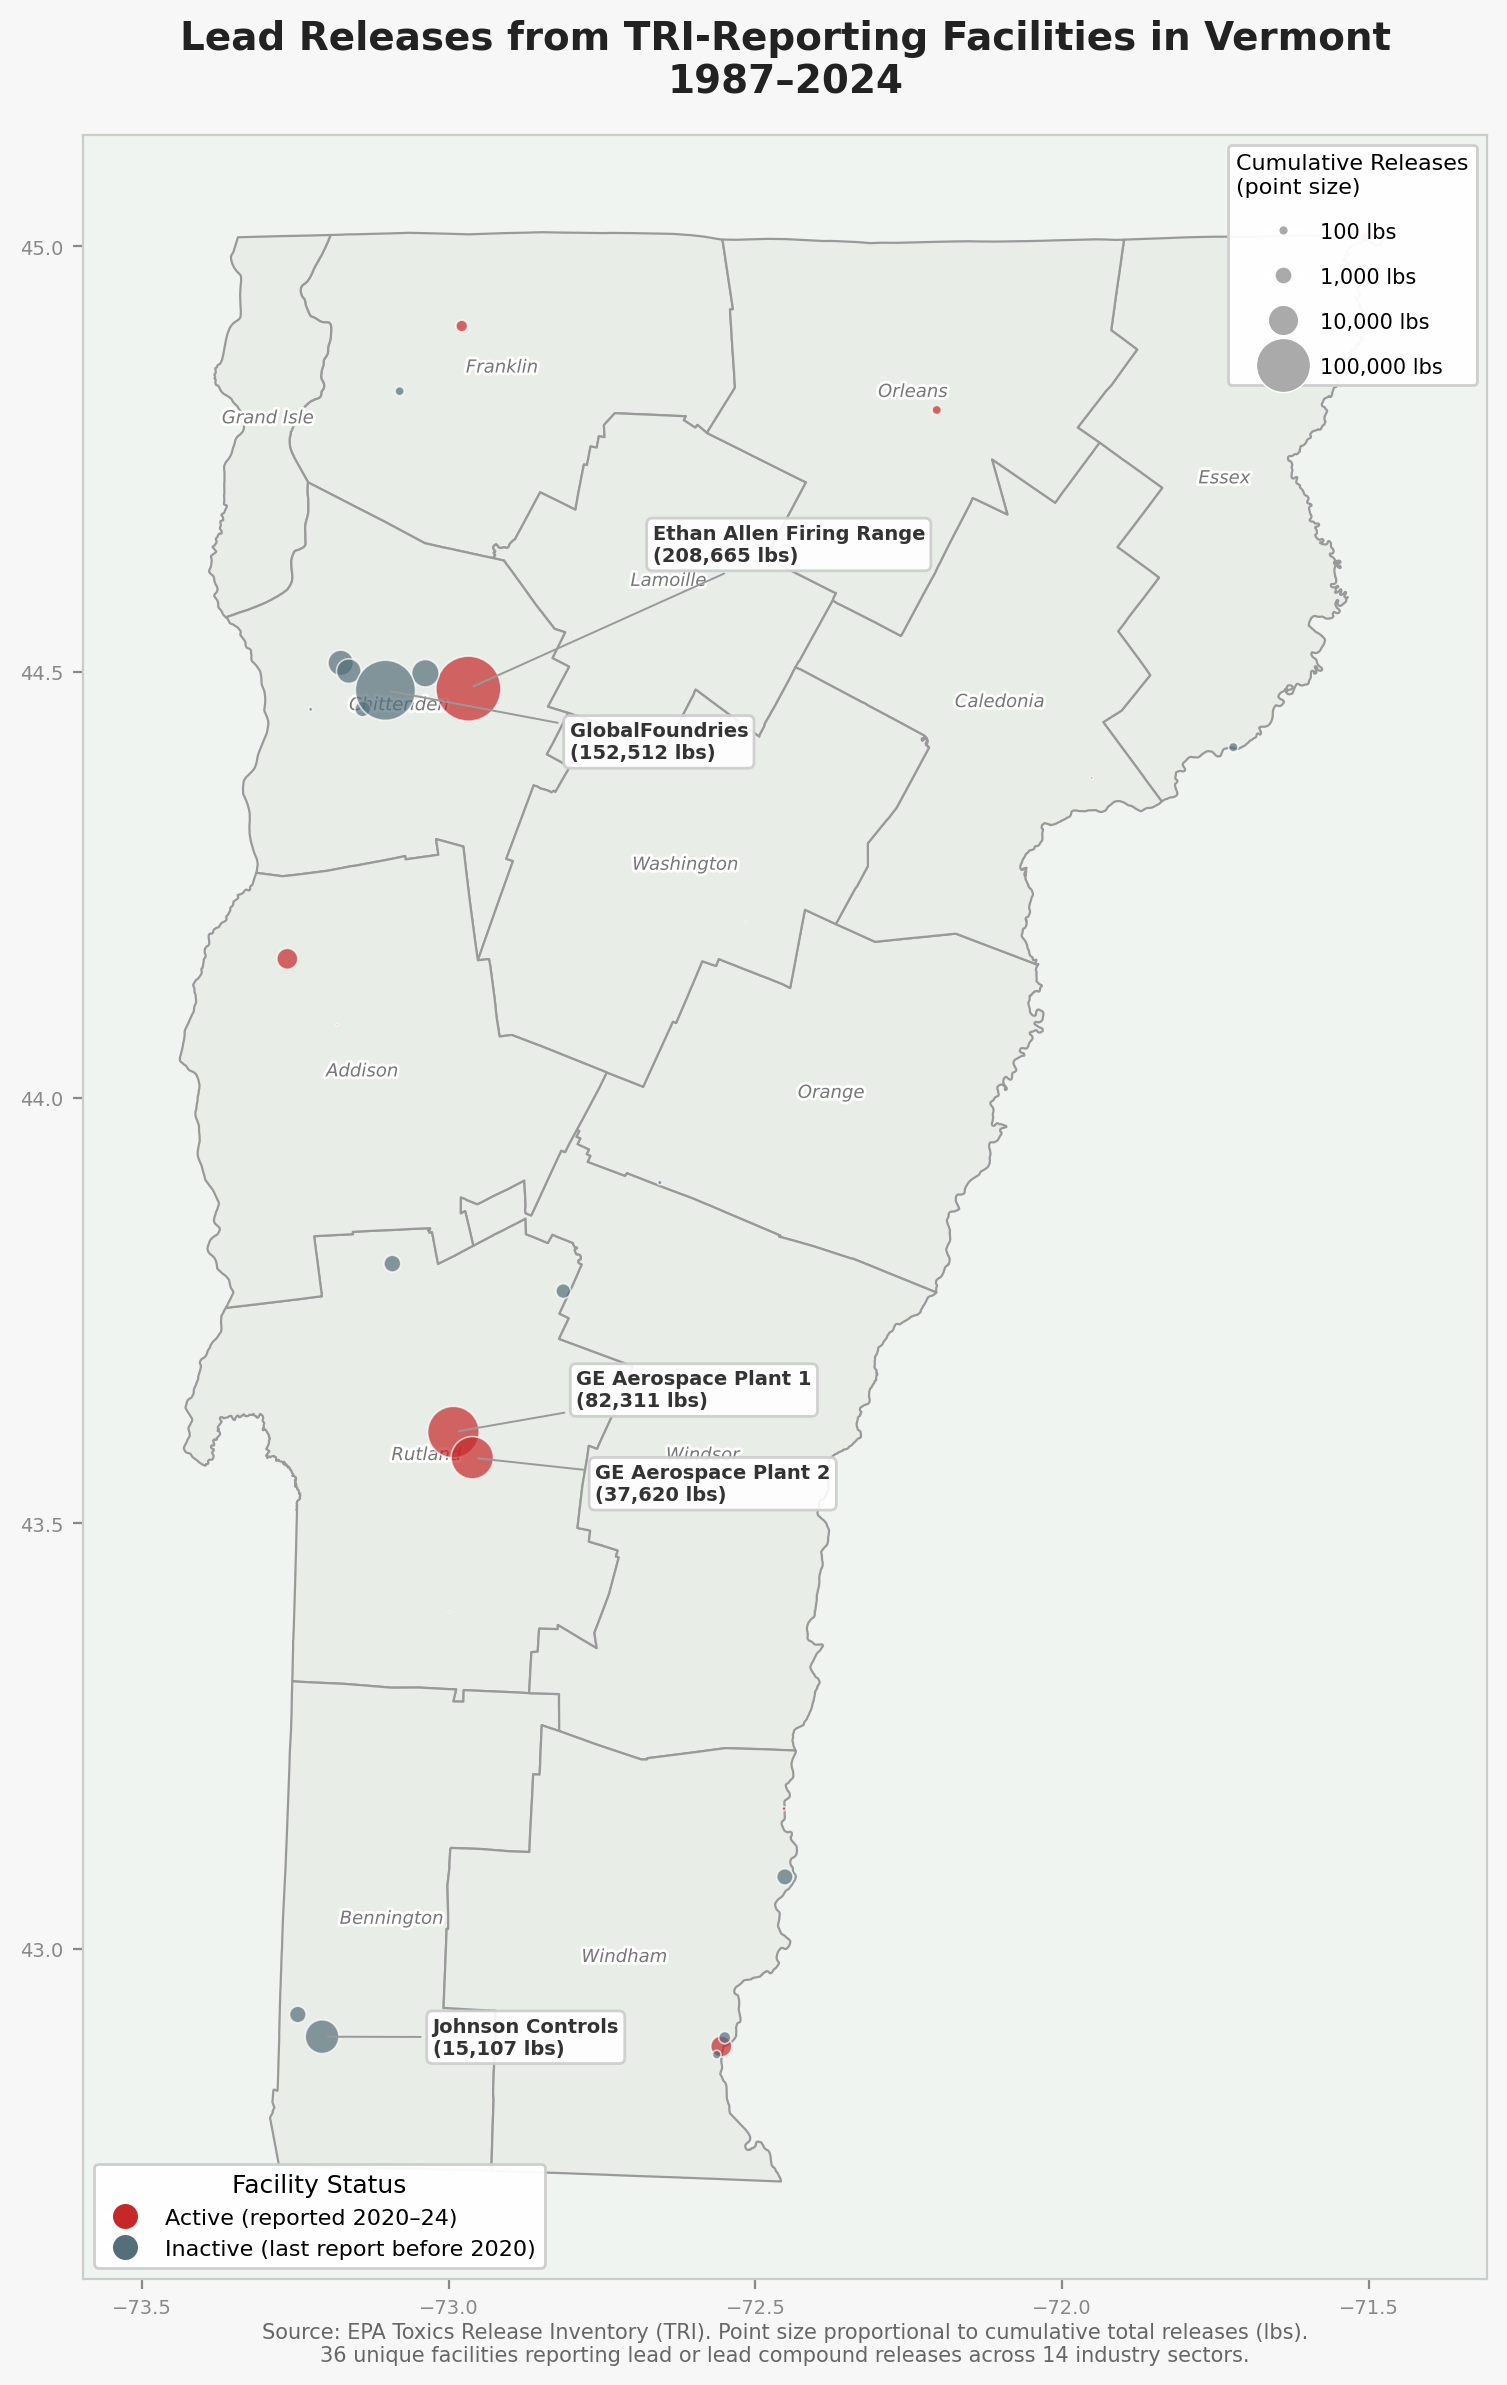
\includegraphics[width=0.85\textwidth, height=0.75\textheight, keepaspectratio]{vt_lead_map.png}
\vskip2pt
{\scriptsize\color{CoolGray} Each dot is a facility. Size = cumulative lead releases (lbs), 1987--2024. Source: EPA TRI.}
\end{frame}

%% ====== SLIDE 9: KEY FINDINGS ======
\begin{frame}{Key Findings: Two Facilities Dominate}
\begin{columns}[T]
\begin{column}{0.55\textwidth}
\vskip2pt
{\small
\begin{tabular}{>{\raggedright\arraybackslash}m{4.8cm} r}
\rowcolor{SlateTeal}
\textcolor{white}{\textbf{Facility}} & \textcolor{white}{\textbf{Lbs}} \\[2pt]
\rowcolor{PaleSage}
Ethan Allen Firing Range & 208,665 \\[2pt]
\rowcolor{white}
GlobalFoundries (Essex Jct) & 152,512 \\[2pt]
\rowcolor{PaleSage}
GE Aerospace Plant 1 (Rutland) & 82,311 \\[2pt]
\rowcolor{white}
GE Aerospace Plant 2 & 37,620 \\[2pt]
\rowcolor{PaleSage}
Johnson Controls (Bennington) & 15,107 \\[2pt]
\end{tabular}
}
\vskip6pt
\begin{tcolorbox}[accentbox, top=3pt, bottom=3pt]
\small Top 2 facilities = \textbf{69\%} of all lead releases.\\
Top 3 = \textbf{85\%}.\\
Total across all facilities: 521,410 lbs.
\end{tcolorbox}
\end{column}
\begin{column}{0.40\textwidth}
\begin{tcolorbox}[quotebox]
\small
The firing range is a National Guard site --- lead from spent ammunition deposited directly into soil. A completely different pollution story than semiconductor manufacturing.
\end{tcolorbox}
\vskip4pt
% EMILY: Add a personal observation here if desired
\begin{tcolorbox}[keybox, title={\faClock\quad Time Trend}]
\scriptsize
Before 2007: industrial off-site transfers.\\
After 2007: military on-site deposition.\\
The \textit{nature} of pollution changed.
\end{tcolorbox}
\end{column}
\end{columns}
\end{frame}

%% ====== SLIDE 10: THE MEMO ======
\begin{frame}{From Curiosity to Written Summary: $\sim$20 Minutes}
\begin{columns}[T]
\begin{column}{0.47\textwidth}
\begin{tcolorbox}[keybox, title={\faFile*[regular]\quad The Summary Memo}]
\small
AI generated a full memo covering:
\begin{itemize}\setlength{\itemsep}{2pt}
  \item Key findings and top facilities
  \item Time trends and compositional shifts
  \item Geographic concentration (2 counties = 95\% of releases)
  \item A real limitations section
\end{itemize}
\vskip2pt
{\scriptsize\color{CoolGray} ``TRI is self-reported, doesn't measure actual exposure, only covers facilities above reporting thresholds.''}
\end{tcolorbox}
\end{column}
\begin{column}{0.47\textwidth}
\begin{tcolorbox}[accentbox]
\small
\textbf{The full pipeline:}
\vskip2pt
\begin{enumerate}\setlength{\itemsep}{1pt}
  \item Describe the data
  \item Propose analysis ideas
  \item I chose the map
  \item AI generated Python code
  \item Reviewed the output
  \item AI wrote the memo
\end{enumerate}
\vskip4pt
\textbf{Total time:} $\sim$20 minutes.\\
\textbf{By hand:} most of a day.
\end{tcolorbox}
\end{column}
\end{columns}
\end{frame}

%% ====== SLIDE 11: GOOD AT VS NOT ======
\begin{frame}{What AI Is Good At Here vs.\ Not}
\vskip-4pt
\begin{columns}[T]
\begin{column}{0.47\textwidth}
\begin{tcolorbox}[keybox, title={\faCheck\quad AI Strengths}, top=3pt, bottom=3pt]
\small
\begin{itemize}\setlength{\itemsep}{2pt}
  \item \textbf{Data orientation} --- reading a CSV, summarizing, catching quirks
  \item \textbf{Code generation} --- the map worked on the first try
  \item \textbf{First-draft reporting} --- memo structure, limitations section
  \item \textbf{Proposing angles} you might not think of
\end{itemize}
\end{tcolorbox}
\end{column}
\begin{column}{0.47\textwidth}
\begin{tcolorbox}[colback=SoftCoral!8, colframe=SoftCoral, boxrule=0.8pt, arc=3pt,
  left=6pt, right=6pt, top=3pt, bottom=3pt,
  fonttitle=\bfseries\small\color{white}, coltitle=white, colbacktitle=SoftCoral,
  title={\faTimes\quad Still Needs You}]
\small
\begin{itemize}\setlength{\itemsep}{2pt}
  \item \textbf{Vermont-specific knowledge} --- Jericho is near residential areas
  \item \textbf{Policy context} --- who uses this, what decisions it informs
  \item \textbf{Deciding what matters} --- 4 ideas, can't tell you which matters for \textit{your} work
\end{itemize}
\end{tcolorbox}
\end{column}
\end{columns}
\vskip4pt
\begin{tcolorbox}[quotebox, width=12cm]
\small The AI is a very fast, very thorough RA who \textbf{just arrived in Vermont last week}. It can do anything you ask, but it doesn't know what to ask.
\end{tcolorbox}
\end{frame}

%% ====== SECTION DIVIDER: DEMO 2 ======
{
\setbeamertemplate{footline}{}
\setbeamercolor{background canvas}{bg=SlateTeal}
\begin{frame}[plain, noframenumbering]
\centering\vfill
{\fontsize{22}{28}\bfseries\selectfont\color{white} Demo 2}\\[6pt]
{\color{UVMGold}\rule{5cm}{0.8pt}}\\[6pt]
{\normalsize\color{UVMGold} Code Audit \& Paper Audit}\\[4pt]
{\small\color{PaleSage} Bangladesh Remote Education RCT}
\vfill
\end{frame}
}

%% ====== SLIDE 12: THE PROBLEM ======
\begin{frame}{The Problem}
\begin{columns}[T]
\begin{column}{0.55\textwidth}
\vskip4pt
\begin{itemize}\setlength{\itemsep}{6pt}
  \item Paper on remote education in Bangladesh
  \item Evaluates TV instruction, adaptive edtech, data subsidies, and teacher support during COVID-era school closures
  \item \textbf{Keeps getting rejected} --- 8 submissions, 11 referee reports
  \item Used AI two ways:
    \begin{itemize}
      \item Clean up the code
      \item Stress-test the paper
    \end{itemize}
\end{itemize}
\end{column}
\begin{column}{0.40\textwidth}
\begin{tcolorbox}[accentbox]
\small
\textbf{Two use cases:}
\vskip4pt
\textbf{1. Code audit}\\
Restructure 3 years of accumulated code into a clean replication package
\vskip4pt
\textbf{2. Paper audit}\\
Adversarial review before resubmission --- catch what referees would catch
\end{tcolorbox}
\end{column}
\end{columns}
\end{frame}

%% ====== SLIDE 13: CODE AUDIT — BEFORE ======
\begin{frame}{Code Audit: Before}
\vskip-4pt
\begin{columns}[T]
\begin{column}{0.47\textwidth}
\begin{tcolorbox}[colback=DarkSlate, colframe=SoftCoral, boxrule=0.8pt, arc=2pt,
  left=4pt, right=4pt, top=3pt, bottom=3pt]
{\color{CoolGray}\ttfamily\tiny
02\_Do files/\\
\quad 01\_master\_5th June 2021.do\\
\quad 03\_vargen\_07sep.do\\
\quad 03\_vargen.do\\
\quad 05\_endline balance\_eb.do\\
\quad 05\_endline balance.do\\
\quad 09\_attrition\_8 July\_e.do\\
\quad 09\_attrition\_8 July.do\\
\quad ...\\
\quad Archive/ {\color{CoolGray!50}(18 files)}\\
\quad WB Submission Files/ {\color{CoolGray!50}(14 copies)}
}
\end{tcolorbox}
\end{column}
\begin{column}{0.47\textwidth}
{\small\color{SoftCoral}\textbf{The problems:}}
\vskip3pt
\small
\begin{itemize}\setlength{\itemsep}{2pt}
  \item \textbf{51 do-files} across 4 subdirectories
  \item Master file from \textbf{June 2021} --- 3 years stale
  \item Date-in-filename: \texttt{\_07sep}, \texttt{\_02July1130am}
  \item Author-in-filename: \texttt{\_eb}, \texttt{\_e}
  \item Hardcoded paths --- only runs on my machine
  \item No documentation, no version control
\end{itemize}
\vskip3pt
\begin{tcolorbox}[quotebox, top=2pt, bottom=2pt]
\scriptsize This is \textbf{extremely common} in economics.
\end{tcolorbox}
\end{column}
\end{columns}
\end{frame}

%% ====== SLIDE 14: CODE AUDIT — AFTER ======
\begin{frame}{Code Audit: After}
\vskip-4pt
\begin{columns}[T]
\begin{column}{0.47\textwidth}
{\scriptsize
\begin{tabular}{>{\raggedright\arraybackslash}m{2.8cm} >{\centering\arraybackslash}m{1.5cm} >{\centering\arraybackslash}m{1.5cm}}
\rowcolor{SlateTeal}
\textcolor{white}{\textbf{Dimension}} & \textcolor{white}{\textbf{Before}} & \textcolor{white}{\textbf{After}} \\[1pt]
\rowcolor{PaleSage}
Do-files & 51 & \textbf{8} \\[1pt]
\rowcolor{white}
Master file & 2021 & Current \\[1pt]
\rowcolor{PaleSage}
Config system & None & Template \\[1pt]
\rowcolor{white}
Version control & None & Git \\[1pt]
\rowcolor{PaleSage}
Documentation & None & Full \\[1pt]
\rowcolor{white}
``Which version?'' & Constant & \textbf{Zero} \\[1pt]
\end{tabular}
}
\vskip3pt
\begin{tcolorbox}[accentbox, top=2pt, bottom=2pt]
\scriptsize \textbf{86 old variants} preserved in Archive/ --- nothing deleted, fully reversible.
\end{tcolorbox}
\end{column}
\begin{column}{0.47\textwidth}
\begin{tcolorbox}[colback=DarkSlate, colframe=DarkSlate, arc=2pt,
  left=4pt, right=4pt, top=2pt, bottom=2pt]
{\color{CoolGray}\ttfamily\tiny
bd-remote-ed/\\
\; code/00\_master\_repo.do\\
\; code/07\_Dofiles\_academic/\\
\;\quad \_globals.do, 02\_datagen.do,\\
\;\quad 03\_vargen.do {\color{UVMGold!70}(THE one)}, ...\\
\;\quad Archive/ {\color{CoolGray!50}(86 old)}\\
\; config/config\_local\_template.do\\
\; docs/ \;\; justfile \;\; README.md
}
\end{tcolorbox}
\vskip3pt
\begin{tcolorbox}[quotebox, top=2pt, bottom=2pt]
\scriptsize \textbf{Time:} $\sim$2 Claude Code sessions (a few hours).
\textbf{By hand:} days, minimum.
\end{tcolorbox}
\end{column}
\end{columns}
\end{frame}

%% ====== SLIDE 15: THE $FLAGS BUG ======
\begin{frame}[fragile]{The Bug: A Copy-Paste Typo Hiding in Plain Sight}
\vskip-2pt
\begin{tcolorbox}[keybox, title={\faBug\quad The \texttt{\$flags} variable list}, top=2pt, bottom=2pt]
\small
\texttt{\$flags} = 17 missing-value indicators used as controls in \textbf{every regression}. Defined independently in 5 scripts.
\end{tcolorbox}
\vskip3pt
\begin{columns}[T]
\begin{column}{0.47\textwidth}
\begin{tcolorbox}[colback=SoftCoral!8, colframe=SoftCoral, boxrule=0.5pt, arc=2pt, left=5pt, right=5pt, top=3pt, bottom=3pt]
\centering{\small\color{SoftCoral}\textbf{3 of 5 scripts (wrong):}}
\vskip3pt
{\ttfamily\small\color{DeepCharcoal}
... \_f\_c\_engaged \_f\_c\_health\\
\colorbox{SoftCoral!20}{\_c\_child\_work}}
\vskip2pt
{\scriptsize Missing the \texttt{\_f\_} prefix}
\end{tcolorbox}
\end{column}
\begin{column}{0.06\textwidth}
\centering\vskip0.8cm
{\large\color{UVMGold}\faArrowRight}
\end{column}
\begin{column}{0.42\textwidth}
\begin{tcolorbox}[colback=PaleSage, colframe=SlateTeal!50, boxrule=0.5pt, arc=2pt, left=5pt, right=5pt, top=3pt, bottom=3pt]
\centering{\small\color{SlateTeal}\textbf{Correct:}}
\vskip3pt
{\ttfamily\small\color{DeepCharcoal}
... \_f\_c\_engaged \_f\_c\_health\\
\colorbox{PaleSage!50}{\_f\_c\_child\_work}}
\end{tcolorbox}
\end{column}
\end{columns}
\vskip3pt
\begin{tcolorbox}[quotebox, top=2pt, bottom=2pt]
\scriptsize \textbf{Result:} \texttt{\_c\_child\_work} appeared \textit{twice} in regressions. The actual missing indicator was left out. Survived 10+ versions across 2+ years. No error, no crash --- just quietly wrong.
\textbf{How AI found it:} cross-referencing every \texttt{global flags} definition across all 51 files.
\end{tcolorbox}
\end{frame}

%% ====== SLIDE 16: WHAT IS /ECON-AUDIT ======
\begin{frame}[fragile]{Paper Audit: What Is \texttt{/econ-audit}?}
\vskip-2pt
\begin{columns}[T]
\begin{column}{0.47\textwidth}
\begin{tcolorbox}[keybox, title={\faSearch\quad Adversarial Review Skill}, top=3pt, bottom=3pt]
\small
A reusable skill that reads a paper and acts as a \textbf{skeptical referee}.
\vskip3pt
\begin{itemize}\setlength{\itemsep}{1pt}
  \item Reads full paper (LaTeX, tables, appendix)
  \item Checks identification, power, measurement
  \item Produces structured audit report
  \item Takes $\sim$60 seconds
\end{itemize}
\end{tcolorbox}
\vskip3pt
\begin{tcolorbox}[colback=DarkSlate, colframe=DarkSlate, arc=2pt,
  left=4pt, right=4pt, top=2pt, bottom=2pt]
{\color{CoolGray}\ttfamily\scriptsize \$ npx skills add eabeam/econ-skills \textbackslash\\
\quad\quad --skill econ-audit}
\end{tcolorbox}
\end{column}
\begin{column}{0.47\textwidth}
\begin{tcolorbox}[accentbox, top=3pt, bottom=3pt]
\small
\textbf{What it checks:}
\vskip3pt
\begin{enumerate}\setlength{\itemsep}{1pt}
  \item \textbf{Identification:} Is the causal claim valid?
  \item \textbf{Statistics:} MHT, power, attrition
  \item \textbf{Measurement:} Are variables measured well?
  \item \textbf{Methodology:} Design consistency
  \item \textbf{Presentation:} Framing, length
\end{enumerate}
\end{tcolorbox}
\end{column}
\end{columns}
\end{frame}

%% ====== SLIDE 17: LIVE DEMO — ECON-AUDIT ======
{
\setbeamercolor{background canvas}{bg=DarkSlate}
\begin{frame}[plain]
\centering\vfill
{\color{UVMGold}\faTerminal\quad\fontsize{12}{14}\selectfont LIVE DEMO}\\[12pt]
{\fontsize{18}{22}\bfseries\selectfont\color{white} Running \texttt{/econ-audit} on the Paper}\\[16pt]
\begin{tcolorbox}[colback=DarkSlate!80, colframe=CoolGray!40, boxrule=0.5pt, arc=3pt,
  left=8pt, right=8pt, top=6pt, bottom=6pt, width=11cm]
{\color{CoolGray}\ttfamily\small\$\; claude}\\[4pt]
{\color{white}\ttfamily\small /econ-audit main.tex}
\end{tcolorbox}
\vskip16pt
{\small\color{CoolGray} Reads the full paper + tables + appendix.}\\[4pt]
{\small\color{CoolGray} Produces a structured audit in $\sim$60 seconds.}\\[8pt]
{\small\color{PaleSage} \faPlay\; Switching to terminal\ldots}
\vfill
\end{frame}
}

%% ====== SLIDE 18: AI AUDIT VS REAL REFEREES ======
\begin{frame}{AI Audit vs.\ Real Referees: 7 of 10 in $\sim$60 Seconds}
\vskip-2pt
{\scriptsize
\begin{tabular}{>{\raggedright\arraybackslash}m{5.5cm} c >{\raggedright\arraybackslash}m{5.2cm}}
\rowcolor{SlateTeal}
\textcolor{white}{\textbf{Referee Criticism}} & \textcolor{white}{\textbf{AI?}} & \textcolor{white}{\textbf{Notes}} \\[2pt]
\rowcolor{PaleSage}
High attrition \& differential attrition & \textcolor{SlateTeal}{\faCheck} & Flagged as Critical; suggested Lee bounds \\[2pt]
\rowcolor{white}
Results don't tell a coherent story & \textcolor{UVMGold}{\faAdjust} & Caught ID problem, missed internal contradictions \\[2pt]
\rowcolor{PaleSage}
Theoretical model not useful & \textcolor{SlateTeal}{\faCheck} & Flagged --- but recommended \textit{including} it \\[2pt]
\rowcolor{white}
Short intervention duration (4--8 weeks) & \textcolor{SoftCoral}{\faTimes} & Requires field knowledge \\[2pt]
\rowcolor{PaleSage}
Noisy learning measures (8-item phone test) & \textcolor{SlateTeal}{\faCheck} & Strong match; flagged IRT minimums \\[2pt]
\rowcolor{white}
Paper too long and hard to follow & \textcolor{SlateTeal}{\faCheck} & Suggested cutting 20--30\% \\[2pt]
\rowcolor{PaleSage}
Multiple hypothesis testing issues & \textcolor{SlateTeal}{\faCheck} & Aggressive; added winner's curse framing \\[2pt]
\rowcolor{white}
Limited external validity / COVID fatigue & \textcolor{UVMGold}{\faAdjust} & Partial; missed publication landscape \\[2pt]
\rowcolor{PaleSage}
Deviations from pre-analysis plan & \textcolor{SlateTeal}{\faCheck} & Caught the spirit, not the specifics \\[2pt]
\rowcolor{white}
Complex randomization hard to interpret & \textcolor{SlateTeal}{\faCheck} & Strong match \\[2pt]
\end{tabular}
}
\vskip3pt
\begin{tcolorbox}[accentbox, top=2pt, bottom=2pt, width=12cm]
\centering\small \textbf{5 full matches, 2 partial, 1 opposite recommendation, 2 misses.}\\
11 referee reports across 8 journals over 4 years --- vs.\ 60 seconds of AI.
\end{tcolorbox}
\end{frame}

%% ====== SLIDE 19: WHAT THE AI MISSED ======
\begin{frame}{What the AI Missed --- And Why It Matters}
\begin{columns}[T]
\begin{column}{0.47\textwidth}
\begin{tcolorbox}[colback=SoftCoral!8, colframe=SoftCoral, boxrule=0.8pt, arc=3pt,
  left=6pt, right=6pt, top=4pt, bottom=4pt,
  fonttitle=\bfseries\small\color{white}, coltitle=white, colbacktitle=SoftCoral,
  title={\faTimes\quad The Misses}]
\small
\begin{itemize}\setlength{\itemsep}{4pt}
  \item \textbf{Short duration:} 4--8 weeks is unusually short for an education RCT. Requires knowing field norms.
  \item \textbf{Internal contradictions:} Data arm increased tutoring \textit{more} than info arm, but only info improved learning. Referees caught this; AI didn't.
  \item \textbf{COVID fatigue:} ``We've seen too many of these papers.'' AI can't know the publication landscape.
\end{itemize}
\end{tcolorbox}
\end{column}
\begin{column}{0.47\textwidth}
\begin{tcolorbox}[quotebox]
\small
\textbf{The opposite advice:}\\[3pt]
The AI recommended \textit{including} the conceptual model. Every referee wanted it \textbf{cut}.
\vskip4pt
Sometimes AI gives exactly the wrong recommendation because it lacks field conventions.
\end{tcolorbox}
\vskip4pt
\begin{tcolorbox}[accentbox]
\small
\textbf{Pattern:}\\[2pt]
AI catches \textbf{statistical/econometric} issues reliably.\\[2pt]
AI misses \textbf{field knowledge}, \textbf{within-paper logic checks}, and \textbf{publication strategy}.
\end{tcolorbox}
\end{column}
\end{columns}
\end{frame}

%% ====== SLIDE 20: HONEST TAKEAWAY ======
\begin{frame}{Takeaway: A Very Good Pre-Submission Check}
\begin{columns}[T]
\begin{column}{0.50\textwidth}
\begin{tcolorbox}[keybox, title={\faCheck\quad What It Replaces}]
\small
\begin{itemize}\setlength{\itemsep}{3pt}
  \item The first 80\% of what a careful internal seminar discussant would say
  \item Catches the systematic stuff: identification, power, MHT, attrition
  \item In one minute, not one month
\end{itemize}
\end{tcolorbox}
\end{column}
\begin{column}{0.44\textwidth}
\begin{tcolorbox}[colback=SoftCoral!8, colframe=SoftCoral, boxrule=0.5pt, arc=3pt,
  left=6pt, right=6pt, top=4pt, bottom=4pt]
\small
\textbf{What it doesn't replace:}
\vskip3pt
\begin{itemize}\setlength{\itemsep}{2pt}
  \item Field-specific intuition
  \item ``Does this make sense given what we know about Bangladesh?''
  \item Publication strategy advice
  \item Colleagues who know your work
\end{itemize}
\end{tcolorbox}
\end{column}
\end{columns}
\vskip8pt
\begin{tcolorbox}[quotebox, width=13cm]
\small \textbf{For the code audit:} it found bugs I didn't find in two years. That alone justified the time.\\[2pt]
\textbf{For the paper audit:} run it before you send a paper out. It's free. It catches the embarrassing stuff.
\end{tcolorbox}
\end{frame}

%% ====== SECTION DIVIDER: CLOSING ======
{
\setbeamertemplate{footline}{}
\setbeamercolor{background canvas}{bg=SlateTeal}
\begin{frame}[plain, noframenumbering]
\centering\vfill
{\fontsize{22}{28}\bfseries\selectfont\color{white} What to Try First}\\[6pt]
{\color{UVMGold}\rule{5cm}{0.8pt}}\\[6pt]
{\normalsize\color{UVMGold} Start Small, Check Each Step}
\vfill
\end{frame}
}

%% ====== SLIDE 21: WHAT TO TRY FIRST ======
\begin{frame}{What to Try First}
\vskip2pt
{\small
\begin{tabular}{>{\centering\arraybackslash}m{0.6cm} >{\raggedright\arraybackslash}m{4.5cm} >{\centering\arraybackslash}m{1.5cm} >{\raggedright\arraybackslash}m{5cm}}
\rowcolor{SlateTeal}
\textcolor{white}{\textbf{\#}} & \textcolor{white}{\textbf{Activity}} & \textcolor{white}{\textbf{Time}} & \textcolor{white}{\textbf{What You Get}} \\[2pt]
\rowcolor{PaleSage}
1 & Create a voice file & 15 min & Your tone in every AI draft --- reuse forever \\[2pt]
\rowcolor{white}
2 & Data pipeline (describe $\rightarrow$ propose $\rightarrow$ code) & 30 min & Orientation on any dataset \\[2pt]
\rowcolor{PaleSage}
3 & Install \texttt{/econ-audit}, run on a paper & 10 min & Pre-submission check for free \\[2pt]
\rowcolor{white}
4 & Try inbox triage with Gmail integration & 30 min & Sorted, triaged, draft replies \\[2pt]
\end{tabular}
}
\vskip8pt
\begin{tcolorbox}[quotebox, width=12cm]
\small All four use the same principle: \textbf{AI does the mechanical parts, you check each step.} Start with whichever one matches a task you already have.
\end{tcolorbox}
\end{frame}

%% ====== SLIDE 22: RESOURCES ======
\begin{frame}{Resources}
\begin{columns}[T]
\begin{column}{0.47\textwidth}
\begin{tcolorbox}[keybox, title={\faLink\quad Links}]
\small
\begin{itemize}\setlength{\itemsep}{4pt}
  \item \textbf{Bootcamp website:}\\{\scriptsize\ttfamily eabeam.github.io/uvmecon-ai}
  \item \textbf{Skills library:}\\{\scriptsize\ttfamily skills.sh}
  \item \textbf{Econ skills:}\\{\scriptsize\ttfamily github.com/eabeam/econ-skills}
  \item \textbf{Claude Code docs:}\\{\scriptsize\ttfamily docs.anthropic.com/en/docs/claude-code}
\end{itemize}
\end{tcolorbox}
\end{column}
\begin{column}{0.47\textwidth}
\begin{tcolorbox}[keybox, title={\faTerminal\quad Install Commands}]
\small
\textbf{Step 1:} Install Node.js\\
{\scriptsize\ttfamily nodejs.org} $\rightarrow$ click LTS\\[4pt]
\textbf{Step 2:} Install Claude Code\\
{\scriptsize\ttfamily npm install -g @anthropic-ai/claude-code}\\[4pt]
\textbf{Step 3:} Install econ skills\\
{\scriptsize\ttfamily npx skills add eabeam/econ-skills}\\[4pt]
\textbf{Step 4:} Launch\\
{\scriptsize\ttfamily claude}
\end{tcolorbox}
\end{column}
\end{columns}
\end{frame}

%% ====== CLOSING SLIDE ======
{
\setbeamertemplate{footline}{}
\begin{frame}[plain]
\begin{tikzpicture}[remember picture, overlay]
  % SlateTeal background matching title slide
  \fill[SlateTeal] (current page.north west) rectangle (current page.south east);
  % Gold accent line
  \fill[UVMGold] ([yshift=0.3cm]current page.center -| current page.west) rectangle ([yshift=0.25cm]current page.center -| current page.east);
  % Thank you (above line)
  \node[text=white, font=\fontsize{28}{34}\bfseries\selectfont, anchor=center]
    at ([yshift=2.2cm]current page.center) {Thank You!};
  \node[text=UVMGold, font=\fontsize{15}{20}\selectfont, anchor=center]
    at ([yshift=1.2cm]current page.center) {Now over to Erkmen};
  % Below the line
  \node[text=white, font=\large\bfseries, anchor=center]
    at ([yshift=-0.6cm]current page.center) {Erkmen G. Aslim \quad\&\quad Emily Beam};
  \node[text=PaleSage, font=\normalsize, anchor=center]
    at ([yshift=-1.3cm]current page.center) {Department of Economics, University of Vermont};
  % URL
  \node[text=CoolGray!70!white, font=\small, anchor=center]
    at ([yshift=-2.2cm]current page.center) {Bootcamp materials \& resources:};
  \node[text=UVMGold, font=\small\ttfamily, anchor=center]
    at ([yshift=-2.8cm]current page.center) {eabeam.github.io/uvmecon-ai};
  % Watermark
  \node[text=white, opacity=0.04, font=\fontsize{100}{100}\selectfont, anchor=center, rotate=15]
    at ([xshift=-4.5cm, yshift=1.5cm]current page.center) {\faRobot};
\end{tikzpicture}
\end{frame}
}

\end{document}
